% Generated by build_paper.py from eon-whitepaper.md.
% Edit Markdown, then regenerate; do not edit this file independently.
\documentclass[11pt,a4paper]{article}
\usepackage{iftex}
\ifPDFTeX
  \usepackage[T1]{fontenc}
  \usepackage[utf8]{inputenc}
\else
  \usepackage{fontspec}
\fi
\usepackage{lmodern}
\usepackage[margin=1in]{geometry}
\usepackage{microtype}
\usepackage{graphicx}
\makeatletter
\define@key{Gin}{alt}{}
\makeatother
\usepackage{float}
\usepackage{placeins}
\usepackage{flafter}
\usepackage[font=small,labelfont=bf,justification=raggedright,singlelinecheck=false]{caption}
\usepackage{booktabs,longtable,array,calc}
\usepackage{listings}
\usepackage{xcolor}
\usepackage{amsmath,amssymb}
\usepackage{enumitem}
\usepackage{titlesec}
\usepackage{fancyhdr}
\usepackage{xurl}
\usepackage[hidelinks]{hyperref}
\definecolor{accent}{HTML}{0F766E}
\definecolor{warn}{HTML}{E0605A}
\definecolor{ink}{HTML}{1F2A37}
\definecolor{shade}{HTML}{F1F4F4}
\color{ink}
\pagestyle{fancy}
\fancyhf{}
\fancyhead[L]{\footnotesize Tomorrow's Newspaper}
\fancyhead[R]{\footnotesize\thepage}
\setlength{\headheight}{14pt}
\renewcommand{\headrulewidth}{0.3pt}
\titleformat{\section}{\normalfont\Large\bfseries\color{accent}}{}{0em}{}
\titleformat{\subsection}{\normalfont\large\bfseries}{}{0em}{}
\titlespacing*{\section}{0pt}{2.5ex plus 1ex}{1.4ex}
\titlespacing*{\subsection}{0pt}{2ex plus 1ex}{1ex}
\setcounter{secnumdepth}{-1}
\setcounter{tocdepth}{1}
\setlength{\parindent}{0pt}
\setlength{\parskip}{5pt plus 1pt}
\setlength{\emergencystretch}{3em}
\raggedbottom
\clubpenalty=10000
\widowpenalty=10000
\displaywidowpenalty=10000
\renewcommand{\arraystretch}{1.12}
\renewcommand{\topfraction}{.95}
\renewcommand{\bottomfraction}{.85}
\renewcommand{\textfraction}{.05}
\renewcommand{\floatpagefraction}{.65}
\setlength{\textfloatsep}{14pt plus 2pt minus 2pt}
\setlength{\intextsep}{12pt plus 2pt minus 2pt}
\setlist{nosep,leftmargin=*}
\newcommand{\tightlist}{\setlength{\itemsep}{0pt}\setlength{\parskip}{0pt}}
\newcommand{\passthrough}[1]{#1}
\newcommand{\pandocbounded}[1]{#1}
\lstset{basicstyle=\ttfamily\footnotesize,backgroundcolor=\color{shade},
  frame=none,framesep=6pt,breaklines=true,columns=fullflexible,
  keepspaces=true,showstringspaces=false,breakatwhitespace=false}
\begin{document}
\hypersetup{pageanchor=false}
\begin{titlepage}
\raggedright
\hyphenpenalty=10000
\vspace*{1.5cm}
{\color{accent}\small EREBUS OBSERVATORY NETWORK / EON\par}
\vspace{1cm}
{\fontsize{36}{40}\selectfont\bfseries Tomorrow's Newspaper\par}
\vspace{.8cm}
{\Large The making of EON, a machine that reads annual reports, and an honest test of what it could see\par}
\vspace{1.3cm}
{\large Gabriel George\par}
\vspace{.5cm}
{\large Technical white paper\par}
30 September 2026 · Edition 4\par
\vspace{1.3cm}
{\renewcommand{\arraystretch}{1.5}
\begin{tabular}{@{}r@{\hspace{1.2em}}l@{}}
{\color{warn!80!black}\Large\bfseries 5} & {\small versions, from a folder of scripts to a system}\\
{\color{accent}\Large\bfseries 29,375} & {\small answers from a language model, each one dated}\\
{\color{ink!70}\Large\bfseries 1} & {\small question: could it see ahead?}\\
\end{tabular}\par}
\vfill
\noindent\textcolor{accent}{\rule{\textwidth}{1pt}}
\vspace{.5cm}
{\small I built a machine to read every annual report in the market. This is how it was built,\par
what it read, and whether it had simply read tomorrow's newspaper.}
\end{titlepage}
\hypersetup{pageanchor=true}
\pagenumbering{roman}
\tableofcontents
\clearpage
\pagenumbering{arabic}

\section{Abstract}\label{abstract}

Over seventeen months I built five versions of the same idea: a machine that reads company
annual reports the way a patient analyst would, and writes down what it thinks. It began in May
2025 as a folder of scripts studying thirty years of great companies. It became EON: a system
of downloaders, headless browsers, key rotation, file locks, leases, heartbeats, a SQLite
database, a command line, a web interface and a Discord alarm, all built around one constraint,
a daily quota of model requests. Together the versions stored 29,375 answers from a language
model, including 6,973 three-lens readings of 10-K filings, each ending in a single verdict.

This paper is mostly about how that machine was built and why it needed every part. It is also
about what the machine read, and whether it was right. Graded naively, its BUY calls beat its
SELL calls by 13 percentage points a year. But the model had been trained on the years it was
being graded on: it may have read tomorrow's newspaper. Graded only on what it could not have
known, the edge shrinks; its SELL calls stop working; a score written down in advance pointed
the wrong way; and an options scan turned out to see how far a stock would move, but not which
way.

It was never going to rival Citadel, Point72 or the Medallion Fund. It was worth building
anyway, as a finance project, an AI project and a systems project at once. The paper ends with
a sealed bet: 1,257 verdicts frozen at publication, to be graded in October 2027.

\emph{Research, not investment advice.}

\section{1. A reader for every annual report}\label{a-reader-for-every-annual-report}

Every public company in the United States files a 10-K each year. It is the fullest account a
company gives of itself: what it sells, how it makes money, what could go wrong, what it owes.
The median 10-K in this project runs to 141 pages. Thousands are filed every spring.
Professional analysts read the few they are paid to cover; almost nobody reads the rest.

I wanted a reader that never tires. Give it any filing and it would read the whole thing, ask
the same careful questions every time, and write down what it concluded, so that I could come
back a year later and see whether it had been right. A language model can now read 141 pages in
a minute. The hard part is everything around that minute.

\begin{figure}[!htbp]
\centering
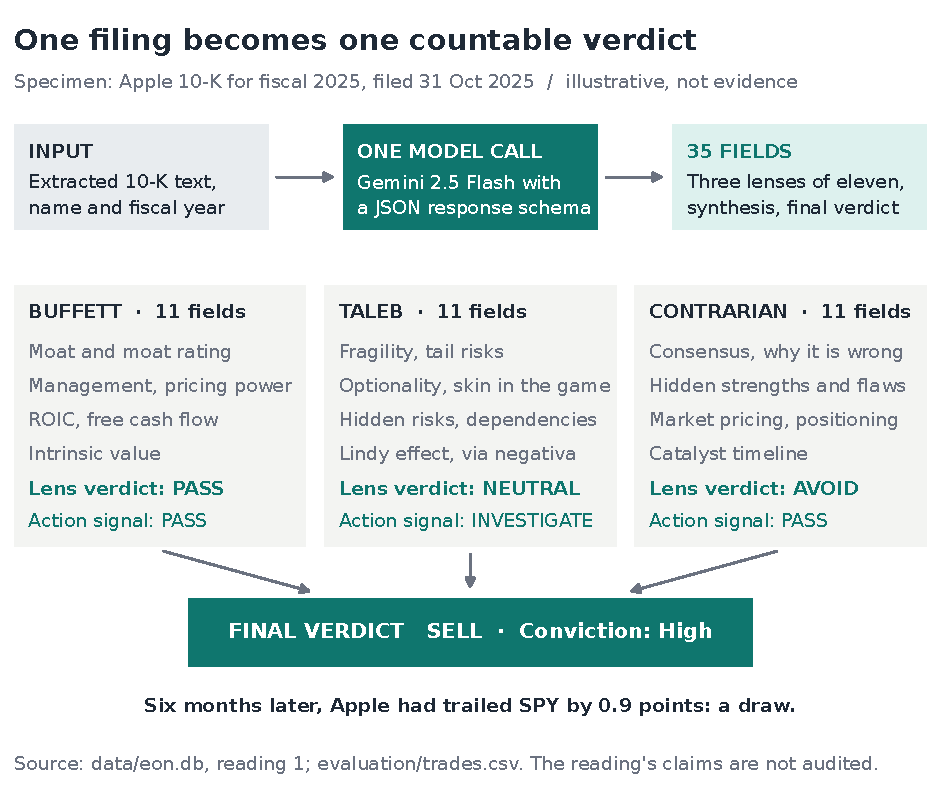
\includegraphics[width=1\linewidth,height=\textheight,keepaspectratio,alt={An Apple 10-K enters one Gemini 2.5 Flash call and returns 35 structured fields: three lenses of eleven, a synthesis, and a final verdict of SELL with high conviction.}]{figures/01-one-reading.pdf}
\caption{One filing becomes one countable verdict. EON's first stored reading: Apple's 10-K for
fiscal 2025, filed 31 October 2025. The model reads the filing as Warren Buffett, Nassim Taleb
and a contrarian would, then gives one verdict. Six months later Apple had trailed the S\&P 500
by 0.9 points: a draw. Sources: data/eon.db; evaluation/trades.csv.}\label{fig:01-one-reading}
\end{figure}

Figure 1 is what the finished machine produces. Its verdict on Apple reads: ``SELL. Conviction:
High. Apple is an undeniably excellent company, but a high conviction SELL rating is warranted
given the significant disconnect between its robust fundamentals and its highly stretched
valuation.'' It is specific, fluent and confident. Whether it is right is a separate question,
and Part II is about how hard that question turned out to be.

The paper has three parts. Part I tells how the machine was built, version by version, and why
each component exists. Part II describes everything it was asked and tests its answers against
what happened. Part III is about what the project taught: where the model failed, and why the
whole thing was worth doing.

\FloatBarrier
\clearpage
\section{Part I · Building the reader}\label{part-i-building-the-reader}

EON was built five times. Each version answered a failure of the last and kept what worked
(Figure 2).

\begin{figure}[!htbp]
\centering
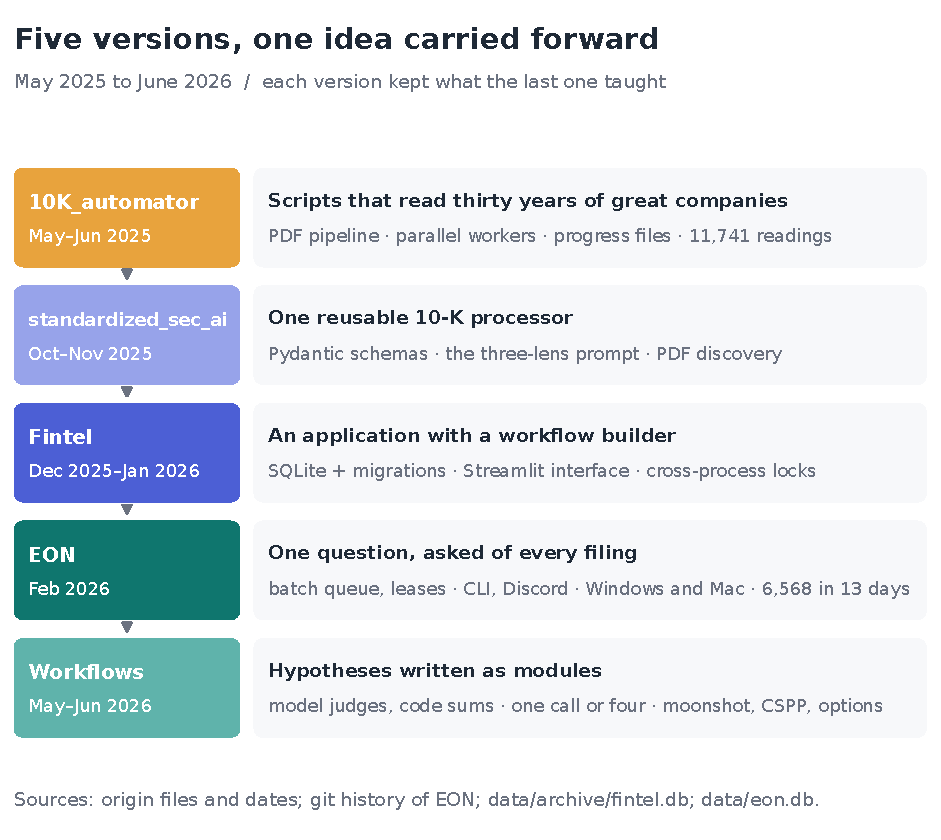
\includegraphics[width=1\linewidth,height=\textheight,keepaspectratio,alt={Five stacked stages from May 2025 to June 2026: 10K\_automator, standardized\_sec\_ai, Fintel, EON and custom workflows, each with what it carried forward.}]{figures/02-lineage.pdf}
\caption{Five versions, one idea carried forward. From scripts studying great companies to an
application that reads every filing. Dates come from the origin project's files and the
repository's git history. Sources: the origin project; git history; data/archive/fintel.db;
data/eon.db.}\label{fig:02-lineage}
\end{figure}

\section{2. The workshop: learning from great companies}\label{the-workshop-learning-from-great-companies}

The project did not begin as a stock picker. It began, in May 2025, as a question about
excellence: what do great companies have in common, and which other companies have it too?

The first answer was a folder of Python scripts called
\passthrough{\lstinline!10K\_automator!}. They downloaded up to thirty years of annual reports
for 39 long-run compounders (Apple, Costco, Copart, Fair Isaac, O'Reilly, AutoZone and others),
converted each one to PDF with a headless Chrome browser, extracted the text, and asked Gemini
2.5 Flash, then an April preview, to describe what made the company work that year. A second
pass distilled each company's thirty readings into success factors; a third distilled all 39
into a meta-analysis.

It found six ``universal'' factors: operational excellence, capital allocation, continuous
innovation, domain expertise, culture, and customer focus. The model credited continuous
innovation to 100\% of the companies. That should have been a warning. A factor that every
great company has, and that nearly every annual report claims, cannot tell great companies from
anyone else.

The scripts then read the recent filings of about 1,900 other companies and scored each from 0
to 100 on its resemblance to the pattern. Between 3 and 13 May they produced 11,741 readings of
individual filings, 4,641 of them on 13 May alone. Two more experiments followed: a contrarian
scan on 26 May, scoring 1,933 companies on six dimensions of hidden strength, and an options
scan on 4 June that proposed 951 trades in calls or puts, run on ten API keys with ten progress
files so that a crash would not lose the day.

Almost everything in EON started in those five weeks: reading whole filings through a browser,
parallel workers, progress files that survive a crash, and the ambition to read the entire
market. So did two problems. The outputs had no fixed format; a script written later to flatten
them found the six success factors spelled about 130 different ways. And the model did not know
what day it was: of 1,919 comparative analyses run in May 2025, 1,916 dated themselves 2024.

The outputs were saved and never changed. More than a year later, that turned out to be their
most valuable property (Section 8.4).

\section{3. From scripts to a processor}\label{from-scripts-to-a-processor}

In October 2025 the scripts became a single reusable module,
\passthrough{\lstinline!standardized\_sec\_ai!}. Its centre was
\passthrough{\lstinline!tenk\_processor.py!}, which downloaded, converted and read filings for
any ticker, and its most important change was a single word: Pydantic.

Pydantic is a Python library for declaring the exact shape of data. Handed to Gemini as a
response schema, it forces the model to answer in named fields of fixed types, and rejects any
answer that does not fit. The project's own notes from that month celebrate it: ``No more JSON
parsing errors!'' The 130 spellings of six factors could not happen again.

The same folder held \passthrough{\lstinline!ppee.py!}, the three-lens prompt from which EON's
is still drawn: read the filing as Buffett would (moat, management, price), as Taleb would
(fragility, tail risk, optionality), and as a contrarian would (what everyone believes, and why
they might be wrong).

\section{4. Fintel: an application}\label{fintel-an-application}

In December 2025 the processor grew into an application called Fintel, with a Streamlit web
interface, a SQLite database and a visual workflow builder. A user could chain steps (pick
companies, fetch filings, run a lens, filter, aggregate, export) and save the chain. The
archive holds 16 of them: comparing three chip makers, reading three nuclear start-ups, pulling
executive pay from a proxy statement.

The builder was good for discovering which questions mattered and bad for measuring anything.
No two chains asked the same thing, so nothing accumulated. It was removed after three weeks.

What stayed was the infrastructure the builder had needed. Fintel was the first version that
ran several analyses at once, and running several analyses at once broke things. Its first rate
limiter used Python's \passthrough{\lstinline!threading.Lock!}, which only works inside one
process. When the command line and the web interface ran together, or a batch spawned several
processes, each had its own lock and the calls collided: the API answered with errors 429 and
503. The fix, recorded in a design note from January 2026, replaced it with a file lock
(\passthrough{\lstinline!portalocker!}) that every process on the machine could see. The same
month brought a nightly queue, an SEC rate limiter, and leases with heartbeats so that a
crashed worker could not strand a company forever.

\section{5. EON: one question, every filing}\label{eon-one-question-every-filing}

In February 2026 the project was renamed EON, the Erebus Observatory Network, and made one
decisive change. Instead of many questions asked of a few companies, it would ask one question
of every company: the three-lens prompt, with a 35-field schema, applied to every listed
company's recent 10-Ks. Essays became a panel, the same measurement taken across 1,358
companies and six fiscal years. Everything in Part II depends on that.

Asking one question of every filing is easy to say. Figure 3 shows what it took.

\begin{figure}[!htbp]
\centering
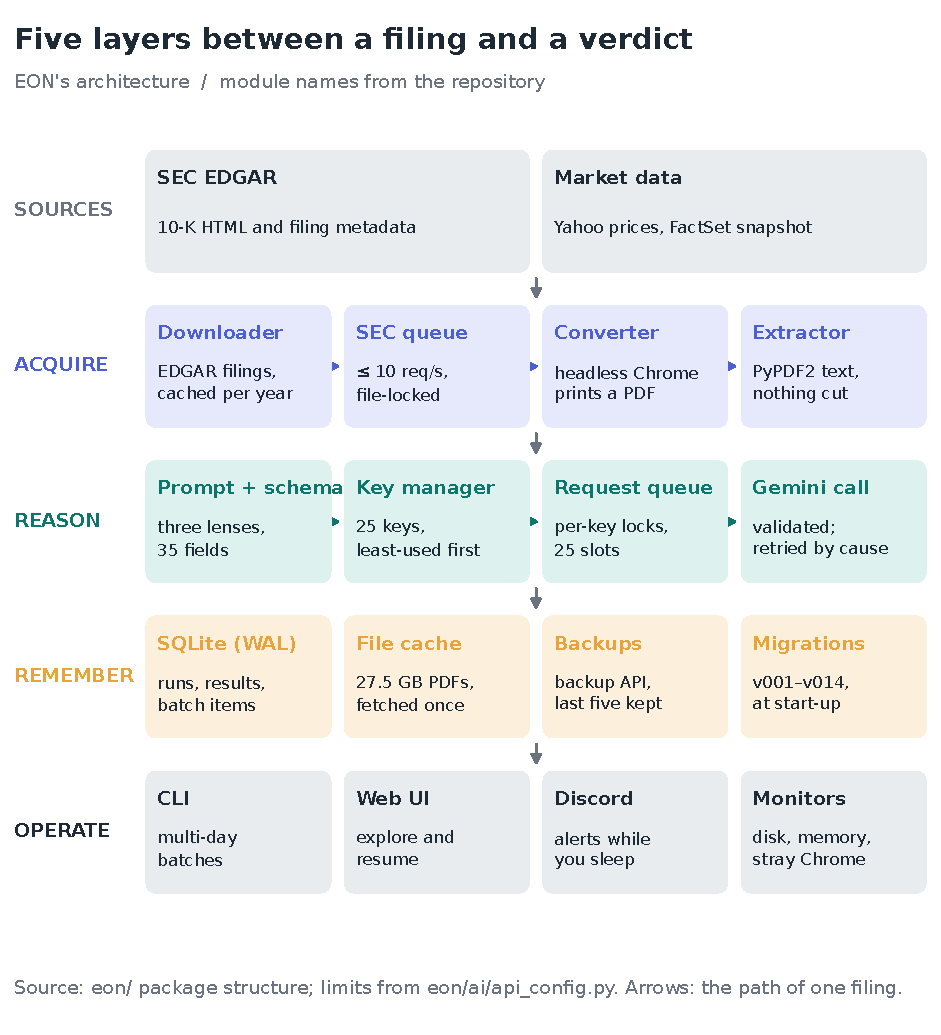
\includegraphics[width=1\linewidth,height=\textheight,keepaspectratio,alt={A layered architecture diagram: sources, acquisition, reasoning, storage and operation layers, with the modules in each.}]{figures/03-architecture.pdf}
\caption{Five layers between a filing and a verdict. Each box is a module in the repository.
Arrows trace one filing: fetched from EDGAR under the SEC's rate policy, printed to PDF by
headless Chrome, extracted to text, sent with the schema through the key manager and request
queue to Gemini, validated, and stored. Source: the eon/ package.}\label{fig:03-architecture}
\end{figure}

Each layer exists because something failed without it. The rest of this section takes them in
turn.

\subsection{5.1 Getting the words: why a PDF, and not XML?}\label{getting-the-words-why-a-pdf-and-not-xml}

The SEC publishes every filing on EDGAR, free, as HTML. EON fetches them with
\passthrough{\lstinline!sec-edgar-downloader!} through its own queue, which keeps well inside
the SEC's fair-access limit of ten requests a second: two seconds between requests, at most
five at once, with a file lock so that parallel workers on one machine share the budget. Each
filing is cached by ticker and year and never fetched twice; the cache now holds 27.5 GB of
PDFs.

Why not simply read the HTML, or use the SEC's machine-readable XBRL data? The measurements
answer both (Figure 4).

\begin{figure}[!htbp]
\centering
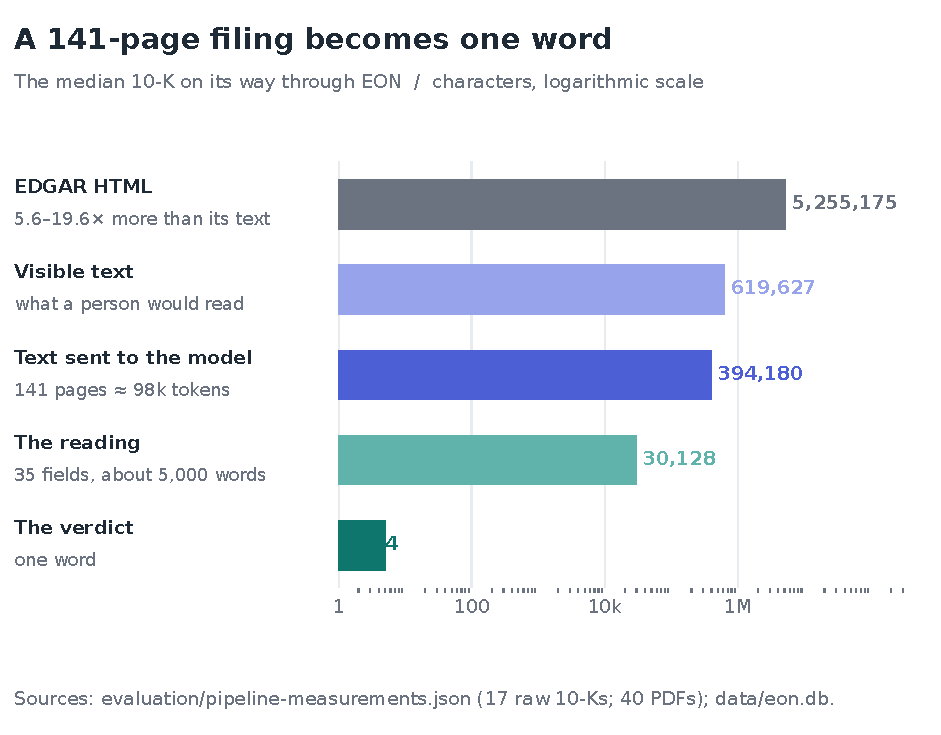
\includegraphics[width=1\linewidth,height=\textheight,keepaspectratio,alt={A logarithmic bar chart of characters at each stage: 5.3 million in the EDGAR HTML, 620,000 visible, 394,000 sent to the model, 30,000 in the reading, and 4 in the verdict.}]{figures/04-life-of-a-filing.pdf}
\caption{A 141-page filing becomes one word. Characters at each stage for the median 10-K: raw
EDGAR HTML across 17 sampled filings, their visible text, the text EON extracts from its PDF
(40 sampled filings), the stored reading, and the verdict. Sources:
evaluation/pipeline-measurements.json; data/eon.db.}\label{fig:04-life-of-a-filing}
\end{figure}

Raw EDGAR HTML is 5.6 to 19.6 times larger than the text a person would read. Most of the
difference is markup, and much of that is inline XBRL: between 1,170 and 3,888 machine-readable
tags per 10-K, plus a hidden header of tagged data. In Kraft Heinz's 2022 10-K, the invisible
XBRL header (645,000 characters) is larger than the entire visible report (642,000). Feed that
HTML to a model and most of what you pay for is markup; strip the tags naively and the hidden
data pours into the text.

XBRL itself is excellent for numbers: revenue, debt, cash flow, tagged and comparable. But
EON's questions are about judgement: moats, fragility, what management says about risk. That
lives in the narrative, which XBRL does not structure.

So EON prints each filing the way a person would see it. A headless Chrome browser opens the
HTML, waits between 3 and 15 seconds depending on the file's size so that the page finishes
rendering, and calls Chrome's own print-to-PDF command. The result is exactly what a reader
sees: tables laid out, hidden XBRL gone, 141 pages at the median. PyPDF2 then extracts the text
in about 6 seconds. Nothing is summarised or cut; a filing too long for the model's context is
skipped, not truncated.

The route costs a browser per filing, and browsers misbehave. A conversion that hangs is
abandoned after 180 seconds and the browser restarted. Orphaned Chrome processes accumulate
over a long batch, so EON sweeps them up every 50 companies, or sooner if memory use passes
80\%. Tables and layout can still be mangled in extraction; that path has not been audited, and
parsing HTML directly would be cleaner. For a machine built to read like a person, printing the
page like a person was the simplest reliable answer.

\subsection{5.2 Asking the question}\label{asking-the-question}

The median filing arrives as about 394,000 characters, roughly 100,000 tokens. EON appends all
of it to the three-lens prompt and sends one request to Gemini 2.5 Flash, with the 35-field
schema attached. The model returns about 30,000 characters, 5,000 words of analysis, and one
verdict (Figure 4).

Pydantic validates every response before it is stored. A response that does not fit is not a
reading. Failures are sorted by cause before they are retried: a rate limit waits for exactly
as long as the API's own retry-after field says; a transient server error backs off and tries
again; a context overflow is marked skipped and never retried. Across all 6,973 three-lens
readings, the model's input came to roughly 0.7 billion tokens.

\subsection{5.3 Twenty requests a day}\label{twenty-requests-a-day}

The binding constraint was not compute, storage or money. It was requests. The February
configuration rotated 25 API keys, each allowed 20 requests a day, with a mandatory 65-second
pause between requests on any one key. That is 500 filings a day, at most.

Every other design decision in EON follows from that number, and getting it right took three
attempts.

The first, in Fintel, was the in-process lock that different processes could not see. The
second was the file lock that fixed it: one lock for the whole machine, held through each
request and its 65-second pause. It worked, and it made 25 keys exactly as slow as one. The
third, in EON, gave every key its own lock file and put a 25-slot semaphore across all of them,
so that 25 requests could run at once while no single key was ever used twice at the same
moment. The pause adapts: it shrinks after a run of successes, down to about 21 seconds, and
grows by half after a rate-limit error.

A fourth bug was quieter. On 6 February 2026 a commit titled ``Remove double-counting of API
key usage that halved effective capacity'' found that every request was recorded twice, once by
the model provider and again by seven of its callers, so each key reached its limit of 20 after
10 real requests. For a while the machine had been running at half speed and reporting itself
full.

Parallelism is what turned 25 keys into 500 readings a day. Figure 5 shows the difference
between the two ways the command line runs.

\begin{figure}[!htbp]
\centering
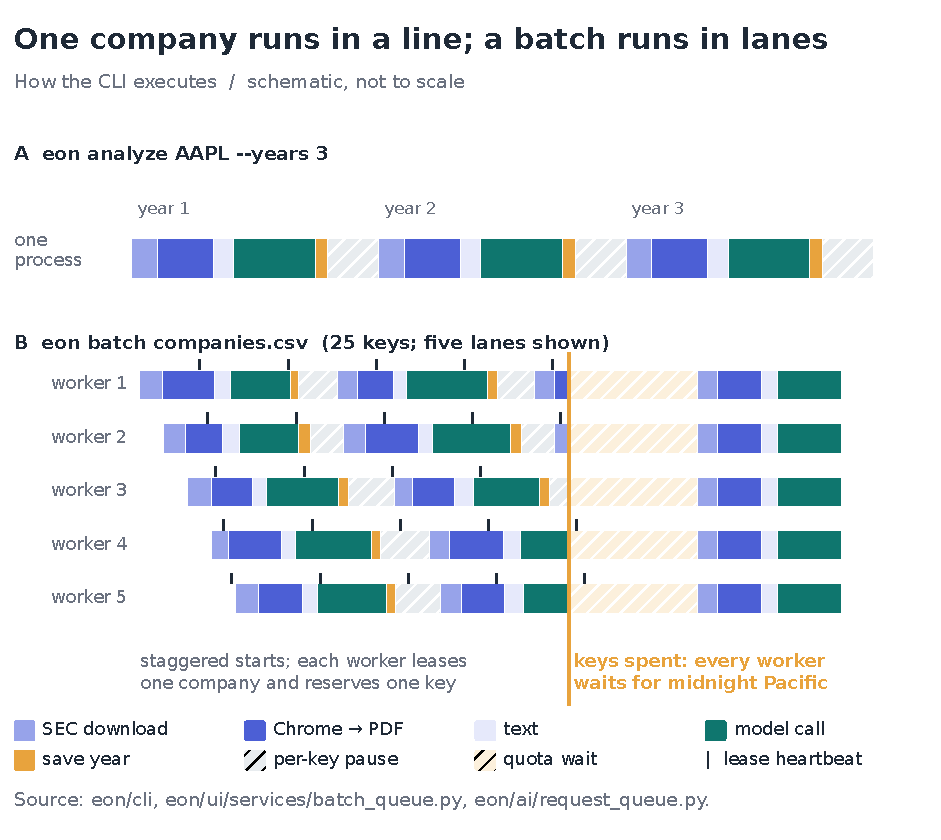
\includegraphics[width=1\linewidth,height=\textheight,keepaspectratio,alt={Two schematic timelines: a single company analysed year by year in one line, and a batch of five workers running staggered in parallel lanes until the daily quota is spent, then waiting for midnight Pacific.}]{figures/05-execution.pdf}
\caption{One company runs in a line; a batch runs in lanes. A single analysis downloads,
prints, extracts, asks and saves one fiscal year after another. A batch starts up to 25 workers
with staggered starts; each leases one company, reserves one key, and renews its lease with a
heartbeat. When every key is spent, all workers wait for the reset at midnight Pacific.
Schematic. Sources: eon/cli; eon/ui/services/batch\_queue.py;
eon/ai/request\_queue.py.}\label{fig:05-execution}
\end{figure}

The market-wide batch ran from 8 to 21 February 2026 and read 6,568 filings from 1,327
companies (Figure 6). At its busiest it finished 189 readings in an hour, one every 19 seconds
across all workers. But it was active for only 62 of the thirteen days' hours. For about 80\%
of its life, the fastest part of the machine was waiting for midnight.

\begin{figure}[!htbp]
\centering
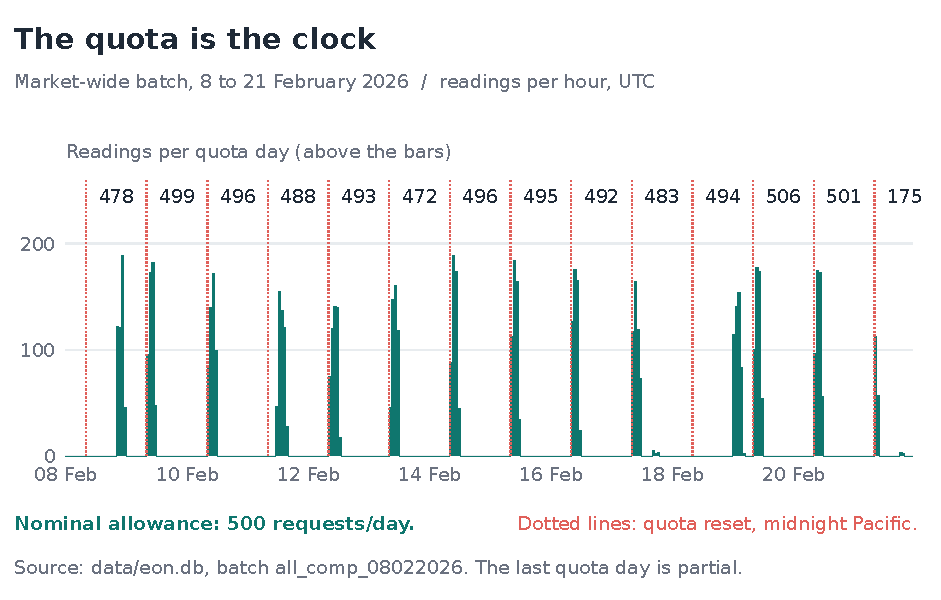
\includegraphics[width=1\linewidth,height=\textheight,keepaspectratio,alt={Hourly readings over fourteen days show a burst after each daily quota reset and near silence in between.}]{figures/06-quota-clock.pdf}
\caption{The quota is the clock. Readings per hour during the February batch, with approximate
quota-day totals of 472 to 506 above the bars. The reset boundary is reconstructed, so a day
can slightly exceed 500. Source: data/eon.db, frozen in
figure-data/evidence.json.}\label{fig:06-quota-clock}
\end{figure}

Of the 1,410 companies attempted, 83 failed: 61 because no filing could be retrieved, and 22
after the model call failed repeatedly.

\subsection{5.4 The database is the batch's memory}\label{the-database-is-the-batchs-memory}

A batch that runs for two weeks will be interrupted: by a crash, a reboot, a power cut, a
closed laptop. The database is what lets it pick up where it left off without losing or
repeating work (Figure 7).

\begin{figure}[!htbp]
\centering
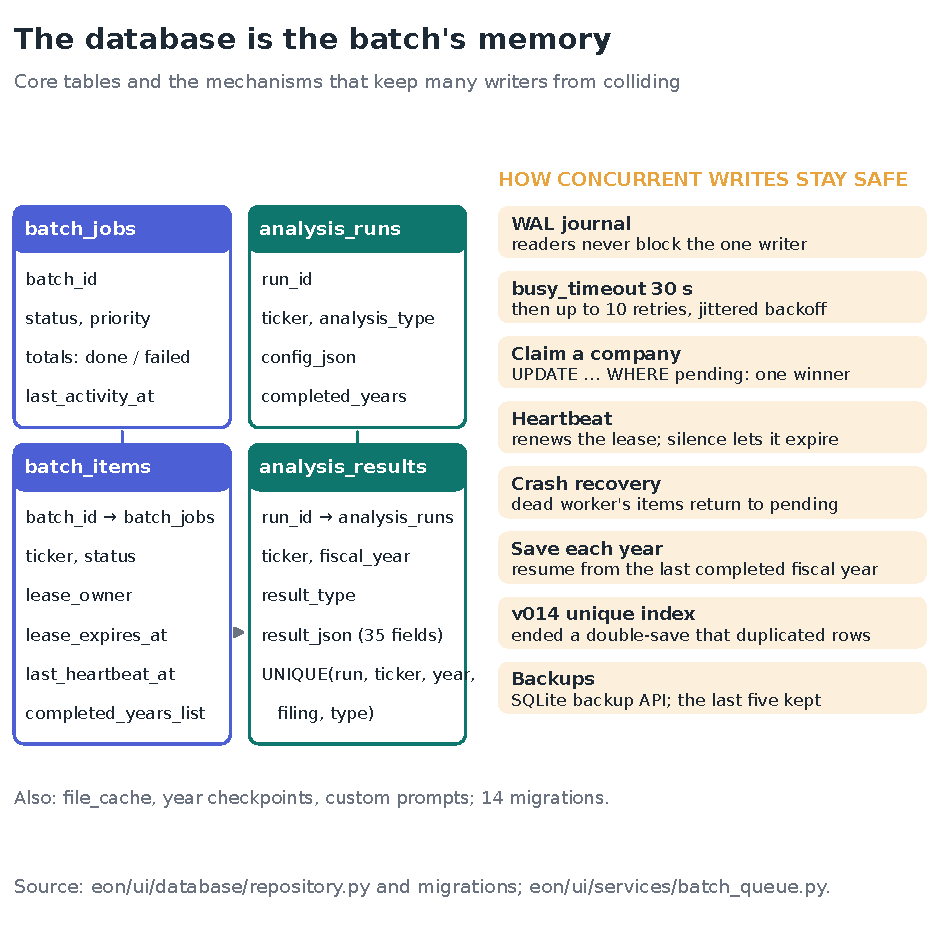
\includegraphics[width=1\linewidth,height=\textheight,keepaspectratio,alt={A diagram of four core tables (batch\_jobs, batch\_items, analysis\_runs, analysis\_results) beside eight mechanisms that keep concurrent writes safe.}]{figures/07-database.pdf}
\caption{The database is the batch's memory. Batch tables track who is working on what;
analysis tables hold what was read. Beside them, the mechanisms that let many workers and two
interfaces share one SQLite file. Sources: eon/ui/database/repository.py and migrations;
eon/ui/services/batch\_queue.py.}\label{fig:07-database}
\end{figure}

EON uses SQLite, a single file, because the whole system runs on one machine and a server
database would add a service to install, configure and keep alive. SQLite's weakness is that
only one writer can write at a time. EON works with that rather than against it.

\begin{itemize}
\tightlist
\item
  \textbf{Write-ahead logging.} In WAL mode readers never block the writer, so the web
  interface can browse results while a batch writes new ones.
\item
  \textbf{Patience, then retries.} Each connection waits up to 30 seconds for the lock, then
  retries up to ten times with exponential backoff and random jitter, so that competing workers
  do not retry in lockstep.
\item
  \textbf{Leases.} A worker claims a company with a conditional update (set it to running, but
  only if it is still pending), so exactly one worker wins. The claim carries a lease of three
  hours, renewed by a heartbeat every five minutes. If a worker dies, its heartbeat stops, its
  lease expires, and the company returns to the queue.
\item
  \textbf{Crash recovery.} On start-up EON checks whether the process that last held the batch
  is still alive. If not, its companies go back to pending.
\item
  \textbf{Per-year checkpoints.} Each fiscal year's reading is saved the moment it arrives. An
  interrupted company resumes from its last completed year, not from the beginning.
\item
  \textbf{A unique index.} In February a double-save pattern (once as each year finished, once
  at the end) quietly stored some readings twice; \passthrough{\lstinline!INSERT OR IGNORE!}
  had nothing to ignore against. Migration 14 removed the duplicates and added a unique index.
  (Separate batches that overlapped still read some company-years twice, which is why 6,973
  stored rows hold 6,653 distinct company-years; the evaluation keeps the first.)
\item
  \textbf{Backups.} During a batch, EON copies the database with SQLite's own backup API and
  keeps the last five.
\end{itemize}

The schema itself has been through 14 migrations, each written to be safe to run twice and
applied automatically at start-up. One earlier file in the repository's history is named
\passthrough{\lstinline!fintel.db.corrupted!}: a reminder of why the rest exists.

\subsection{5.5 Two front doors and a doorbell}\label{two-front-doors-and-a-doorbell}

EON has a command line and a web interface, and they do different jobs.

The command line is for long work. A batch of a thousand companies over ten years needs twenty
days of quota; the README's advice is to start it in a terminal multiplexer and detach, because
a batch must outlive any browser tab. \passthrough{\lstinline!eon batch!},
\passthrough{\lstinline!eon analyze!}, \passthrough{\lstinline!eon export!} and
\passthrough{\lstinline!eon scan-contrarian!} are built with Click.

The Streamlit web interface is for looking: launching a single analysis, browsing history,
reading results, managing the batch queue, and resuming anything interrupted. For a while the
two had their own code paths and drifted apart. On 6 February both were rebuilt on one shared
service layer, so a batch started from either behaves the same way, and a batch started from
the command line can be watched from the browser.

The doorbell is Discord. A batch that runs overnight for two weeks needs a way to say something
while its owner is asleep or away. EON posts to a Discord webhook when a batch completes or
fails, when every key is spent and it is waiting for the reset, and when disk space runs low:
the 27.5 GB of PDFs are a real risk. Before starting, it checks that there is room.

\subsection{5.6 Two machines}\label{two-machines}

EON ran on two computers. The February batch ran on Windows; the database still stores its
paths with backslashes. Development happened on a Mac, which kept its own database of 1,184
readings. A pull request titled ``multi-os support'', merged on 2 February 2026, made the
difference invisible. File locks use \passthrough{\lstinline!portalocker!}, which speaks both
Windows and Unix locking. Paths are built with the platform's own separators. Stray Chrome
processes are cleaned up with \passthrough{\lstinline!pkill!} on the Mac and
\passthrough{\lstinline!taskkill!} on Windows.

\subsection{5.7 Is it efficient?}\label{is-it-efficient}

It depends on what is scarce.

Against the quota, EON is efficient: every request is a whole filing, nothing is sent twice,
and nothing is lost to a crash. Against the clock, it is not: the batch spent about 80\% of its
time waiting. Against compute, it is wasteful but cheap: a browser per filing and about 6
seconds of extraction buy a faithful text. Against storage, it is heavy: 27.5 GB of PDFs for a
database of 240 MB.

If requests were plentiful, the design would change. Parsing HTML directly would drop the
browser. Caching extracted text instead of PDFs would cut the disk. Sending only the sections
each lens needs would cut tokens substantially. Every one of those trades faithfulness for
speed, and while the quota was the constraint, there was no reason to make them.

\section{6. Workflows as hypotheses}\label{workflows-as-hypotheses}

With the panel built, the questions became narrower. From May 2026 new analyses were written as
custom workflows: Python files, discovered automatically, each with its own prompt and schema.
They became a way to write down a hypothesis and test it on hundreds of filings.

\textbf{CSPP} turned a long analytical framework (17 scored components in 5 domains) into a
reading. Its first version asked for everything in one call, with a schema of about 106 KB, 28
times the size of one lens. When any of its roughly 200 required fields drifted, validation
failed and the whole reading was lost. On 20 May 2026 it was split into four smaller calls,
merged in code, with a partial result kept if one part fails. The rewrite also stopped trusting
the model's arithmetic: it supplies component scores, and Python adds them up.

\textbf{Moonshot \ensuremath{\times} Excellence} asked whether a company offers an asymmetric bet and whether it
resembles the great companies of 2025. It uses one call on purpose: it can include up to
250,000 tokens of reference material, and a second call would resend all of it and spend
another request. It rates six dimensions on anchored 0--10 scales and computes the totals in
code. It also carries a watchdog, added after a large filing hung a call for about two hours
without an error.

\textbf{Contrarian Hunter} and the \textbf{options scans} brought the 2025 experiments into
EON. The February 2026 options scan, Asymmetric Options V4, read the latest filing of 1,415
companies in two days and assigned each a directional bias. Section 8.5 tests it.

Two rules came out of this work. Split a question the model cannot answer reliably in one
piece. And let the model judge while code does the counting.

\FloatBarrier
\clearpage
\section{Part II · What it read}\label{part-ii-what-it-read}

\section{7. Every question it was asked}\label{every-question-it-was-asked}

Across five versions, the model gave 29,375 stored answers (Figure 8).

\begin{figure}[!htbp]
\centering
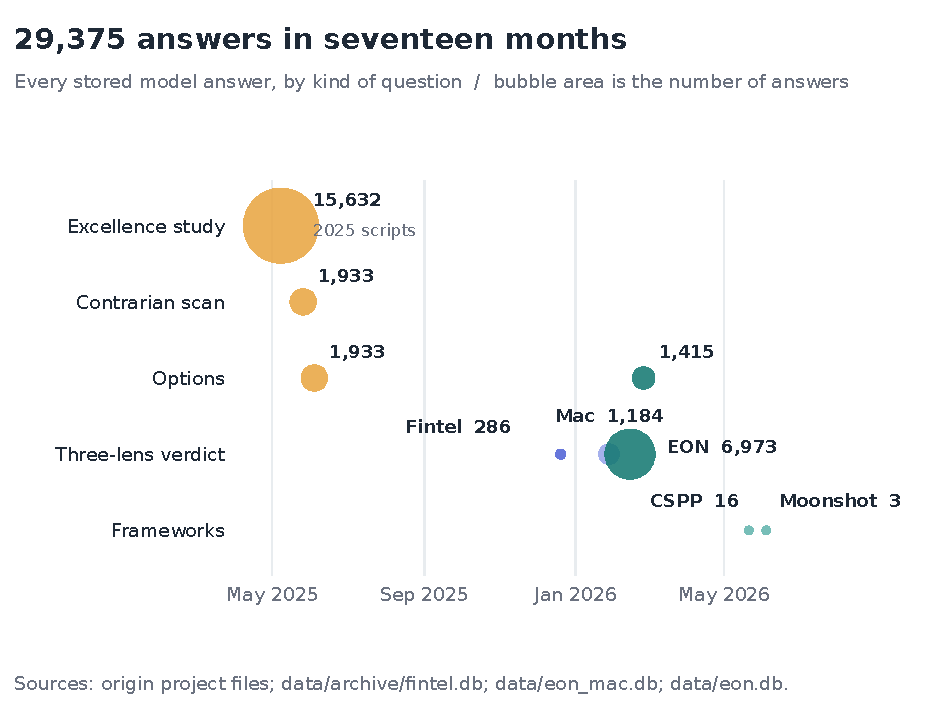
\includegraphics[width=1\linewidth,height=\textheight,keepaspectratio,alt={A bubble timeline from May 2025 to June 2026 showing the answer counts of each kind of analysis: the excellence study, contrarian and options scans, three-lens verdicts, and frameworks.}]{figures/08-catalogue.pdf}
\caption{29,375 answers in seventeen months. Every stored model answer, grouped by the question
it answered. Bubble area is the number of answers. Sources: the origin project's files;
data/archive/fintel.db; data/eon\_mac.db; data/eon.db.}\label{fig:08-catalogue}
\end{figure}

{\def\LTcaptype{table} % do not increment counter
\par\addvspace{8pt}\noindent\begin{minipage}{\linewidth}\small
\begin{tabular}{@{}
  >{\raggedright\arraybackslash}p{(\linewidth - 6\tabcolsep) * \real{0.2200}}
  >{\raggedright\arraybackslash}p{(\linewidth - 6\tabcolsep) * \real{0.2000}}
  >{\raggedleft\arraybackslash}p{(\linewidth - 6\tabcolsep) * \real{0.1100}}
  >{\raggedright\arraybackslash}p{(\linewidth - 6\tabcolsep) * \real{0.4700}}@{}}
\toprule\noalign{}
\begin{minipage}[b]{\linewidth}\raggedright\bfseries
Analysis
\end{minipage} & \begin{minipage}[b]{\linewidth}\raggedright\bfseries
When
\end{minipage} & \begin{minipage}[b]{\linewidth}\raggedleft
Answers
\end{minipage} & \begin{minipage}[b]{\linewidth}\raggedright\bfseries
Asked
\end{minipage} \\
\midrule\noalign{}


Excellence study & May 2025 & 15,632 & What made great companies great, and who resembles
them? \\
Contrarian scan & May 2025 & 1,933 & Where is strength hidden that others miss? \\
Options ideas & June 2025 & 1,933 & Buy calls, buy puts, or neither? \\
Fintel analyses & Dec 2025--Jan 2026 & 286 & Fundamentals, single lenses, syntheses \\
Three-lens verdicts & Jan--Jul 2026 & 8,157 & Buy, hold or sell, as Buffett, Taleb and a
contrarian \\
Asymmetric Options V4 & Feb 2026 & 1,415 & Which way is the tail risk? \\
CSPP and Moonshot & May--Jun 2026 & 19 & Frameworks too large for one call \\
\bottomrule\noalign{}
\end{tabular}
\end{minipage}\par\addvspace{8pt}
}

Read together, the answers show a model with habits.

\begin{itemize}
\tightlist
\item
  \textbf{It likes to hold.} Of 6,411 dated three-lens verdicts, 50.8\% say HOLD, 27.5\% BUY,
  16.5\% SELL, 3.8\% STRONG BUY and 1.4\% STRONG SELL. The mix barely moves from year to year,
  through a boom, a bear market and a recovery. Conviction is Medium 4,632 times, High 1,516
  times and Low only 148 times.
\item
  \textbf{It finds danger everywhere when asked to look for it.} Asked where the tail risk
  lies, the February 2026 options scan gave 873 companies (62\%) a put bias and 27 (2\%) a call
  bias.
\item
  \textbf{It favours the famous.} The 2025 contrarian scan, meant to find hidden gems, put
  MicroStrategy first, followed by Apple, AST SpaceMobile, Tesla, Microsoft and Nvidia. Only 27
  of 1,933 companies scored 70 or more.
\item
  \textbf{Its numbers cluster.} A quarter of all 2025 compounder scores are exactly 68, and
  three values cover 44\% of companies.
\end{itemize}

None of this says whether the answers were right. That takes a test, and the test is harder
than it looks.

\section{8. Was it right?}\label{was-it-right}

\subsection{8.1 Three dates}\label{three-dates}

In February 2026, while the market-wide batch was still running, I checked the readings against
stock returns. BUY-rated filings had beaten SELL-rated ones by 14.1 percentage points over two
years. The report concluded that the model had genuine stock-picking skill.

It had skipped a question. The model was being graded on years it had already read about.
Gemini 2.5 Flash's training data ends in January 2025, according to Google, and this paper uses
31 January 2025 as the line. Show it a 2021 annual report and ask whether to buy: the report
ends in 2021, but the model knows how 2022 went. A backtest like that is a trader handed
tomorrow's newspaper. Their record would be extraordinary, and it would say nothing about their
judgement.

Every verdict therefore has three dates: when the company filed, where the model's knowledge
ends, and when the verdict was written. Their order decides what a test can prove (Figure 9).

\begin{figure}[!htbp]
\centering
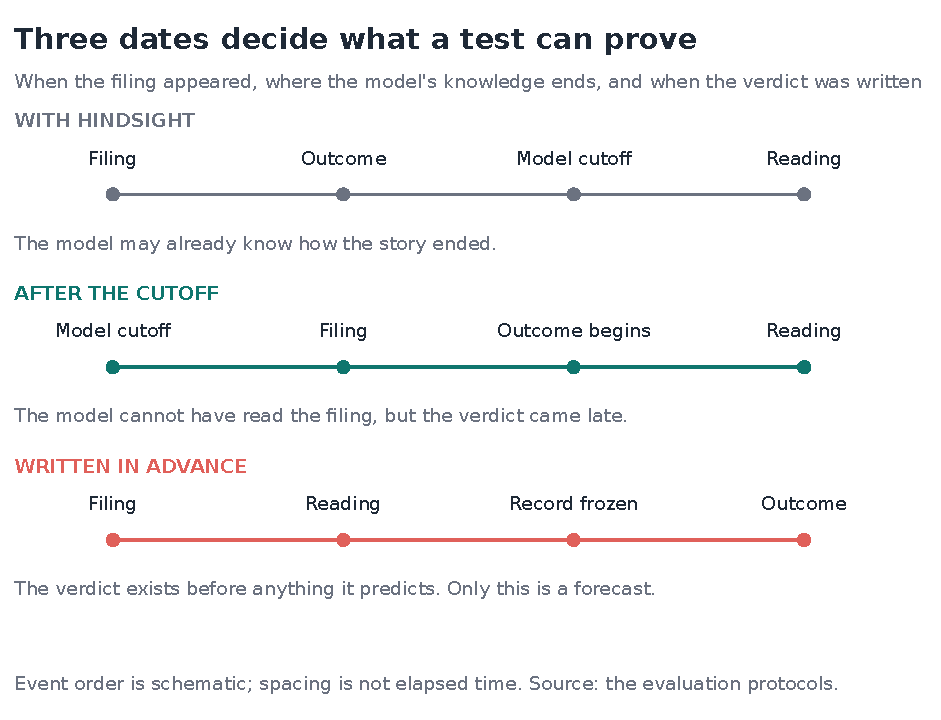
\includegraphics[width=1\linewidth,height=\textheight,keepaspectratio,alt={Three timelines: with hindsight, after the cutoff, and written in advance, showing the order of filing, cutoff, reading and outcome in each.}]{figures/09-three-clocks.pdf}
\caption{Three dates decide what a test can prove. Only the third arrangement, a verdict
recorded before anything it predicts, is a forecast in the ordinary sense. Event order is
schematic. Source: the evaluation protocols.}\label{fig:09-three-clocks}
\end{figure}

Every test below uses one reading per company and year; entry at the first close after the
filing (or, for the ledgers, after the reading); returns in excess of SPY, the S\&P 500 fund;
and significance from shuffling verdicts 10,000 times within each year, and within each year
and industry. Appendix A has the details.

\subsection{8.2 With hindsight, and after the cutoff}\label{with-hindsight-and-after-the-cutoff}

For one-year windows that closed before the cutoff, 1,099 BUY readings beat SPY by 2.2 points
and 657 SELL readings trailed it by 10.9: a spread of 13.1 percentage points (p = 0.0001).
About 42\% of it came from favouring the right industries.

For the 1,443 filings published after the cutoff, which the model cannot have read, the same
test gives a different picture (Figure 10). Ranked by where each stock finished within its
year, the spread halves, from 11.1 to 6.2 percentile points. The average spread, 14.9 points,
looks unchanged, but its uncertainty is ±23 points.

\begin{figure}[!htbp]
\centering
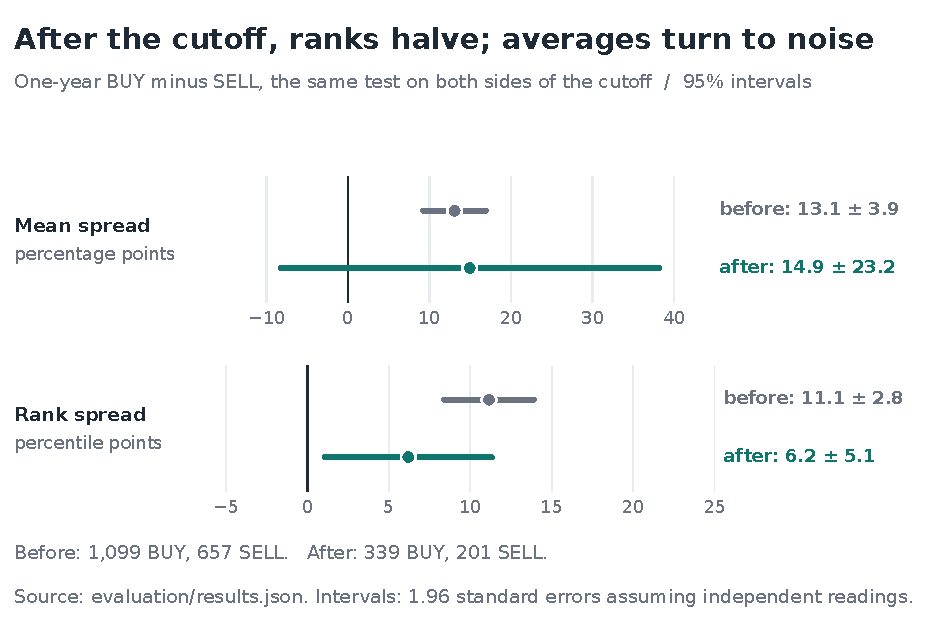
\includegraphics[width=1\linewidth,height=\textheight,keepaspectratio,alt={Two dumbbell rows compare mean and rank spreads before and after the cutoff: the mean is similar but far less certain after; the rank spread halves.}]{figures/10-before-after.pdf}
\caption{After the cutoff, ranks halve; averages turn to noise. The same one-year
BUY-minus-SELL comparison on both sides of the model's knowledge cutoff, with 95\% intervals
from independent-reading standard errors. The permutation tests in the text are the formal
results. Source: evaluation/results.json.}\label{fig:10-before-after}
\end{figure}

Where the edge lived also changed (Figure 11). Before the cutoff, the five verdicts formed a
perfect staircase: STRONG SELL companies finished at the 43rd percentile of their year, SELL at
the 43rd, HOLD at the 50th, BUY at the 54th, STRONG BUY at the 60th. After it, BUY still
finished above the middle, but SELL rose to the 49th percentile, level with HOLD. The SELL
calls, which had carried most of the historical spread, stopped working.

\begin{figure}[!htbp]
\centering
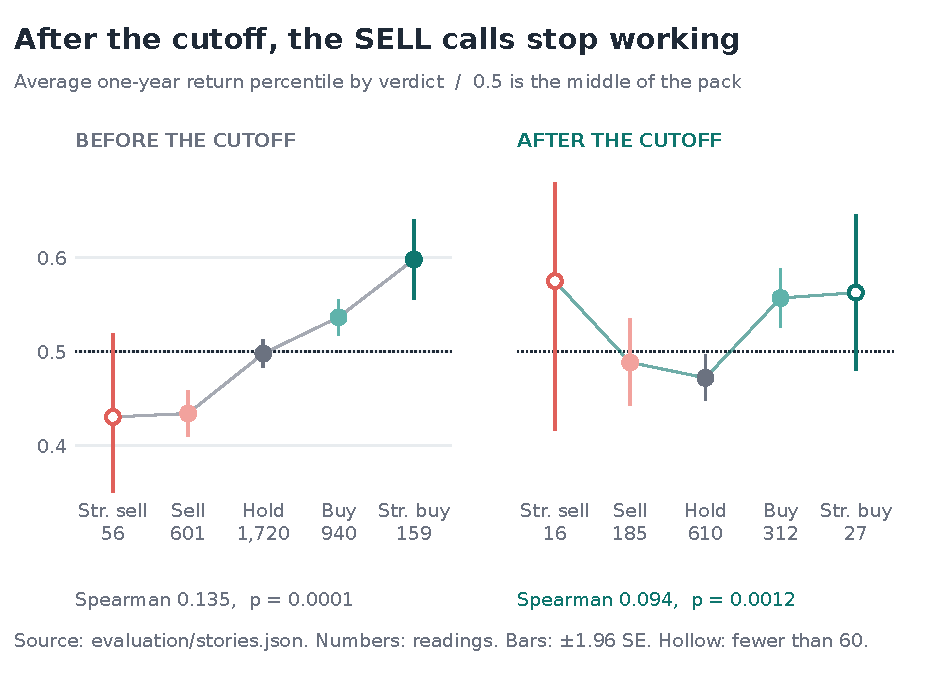
\includegraphics[width=1\linewidth,height=\textheight,keepaspectratio,alt={Two panels show average return percentile by verdict: a steady climb before the cutoff; after it, SELL and HOLD sit together below the middle while BUY stays above.}]{figures/11-verdict-ladder.pdf}
\caption{After the cutoff, the SELL calls stop working. Average within-year percentile of
one-year excess return by verdict, ±1.96 standard errors; hollow points have fewer than 60
readings. The verdict order still correlates with outcomes after the cutoff (Spearman 0.094, p
= 0.0012), driven by BUY rather than SELL. Descriptive. Source:
evaluation/stories.json.}\label{fig:11-verdict-ladder}
\end{figure}

A model that remembered which companies collapsed would look like this. So would a model whose
caution suited 2021 to 2024 and not 2025. The data cannot choose between them.

What survives the cutoff is real but small. By rank, BUY readings beat SELL readings by
\textbf{5.9 percentile points (p = 0.0059)} within industries. That statistic was chosen after
the next figure was seen, and it rests largely on one filing season. By average, the result is
inconclusive: 4.6 points at six months (p = 0.094) and 14.9 at a year (p = 0.215).

\subsection{8.3 One stock, and twenty-four}\label{one-stock-and-twenty-four}

The average fails because of one company (Figure 12). Babcock \& Wilcox filed its 10-K on 31
March 2025, closed at \$0.46 the next day, and stood at \$15.72 a year later: 3,314 points
ahead of SPY. That single reading adds 10 points to the BUY group's average. The price series
was checked against Nasdaq's independent record; there was no split. EON read the filing on 9
February 2026, rated it BUY, and by then the stock had already risen about twentyfold. The
model could not see that: its training ended first, and its call path has web search switched
off.

\begin{figure}[!htbp]
\centering
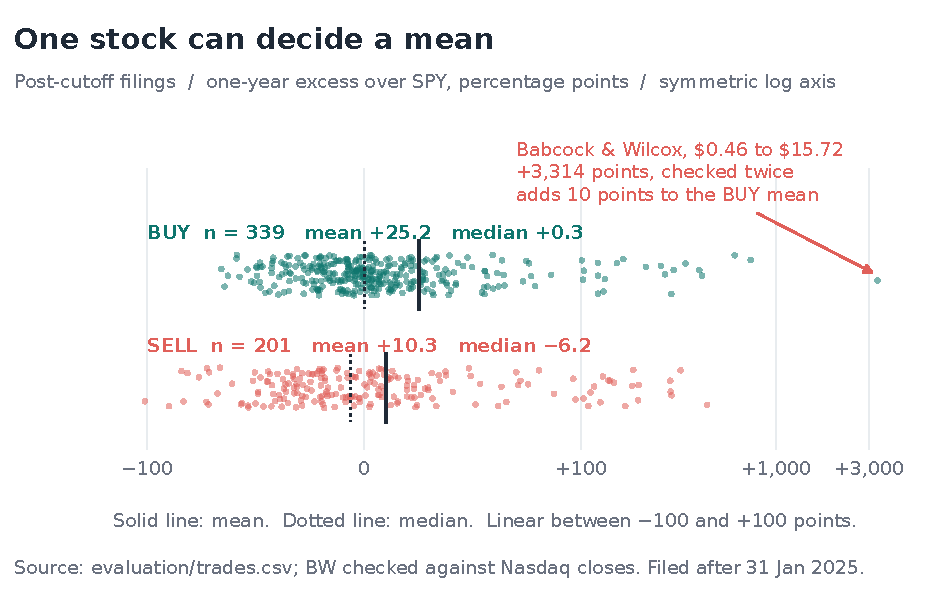
\includegraphics[width=1\linewidth,height=\textheight,keepaspectratio,alt={Strip plot of one-year excess returns after the cutoff: one BUY-rated stock, Babcock \& Wilcox, sits far right at +3,314 points, dragging the BUY mean above its median.}]{figures/12-tails.pdf}
\caption{One stock can decide a mean. Every post-cutoff BUY and SELL reading with a one-year
outcome. Solid lines are means, dotted lines medians; the axis is linear to ±100 points and
logarithmic beyond. Sources: evaluation/trades.csv;
evaluation/verification/bw-price-check.json.}\label{fig:12-tails}
\end{figure}

Averages also hide what the verdicts look like one company at a time. Figure 13 shows 24
companies drawn at random, with a published seed, from the 195 that EON read in every year from
2020 to 2024 and rated both BUY and SELL at least once. Of their 70 BUY and SELL calls, 40 went
the right way: 57\%. Read row by row, the grid looks less like foresight than a slightly loaded
coin.

\begin{figure}[!htbp]
\centering
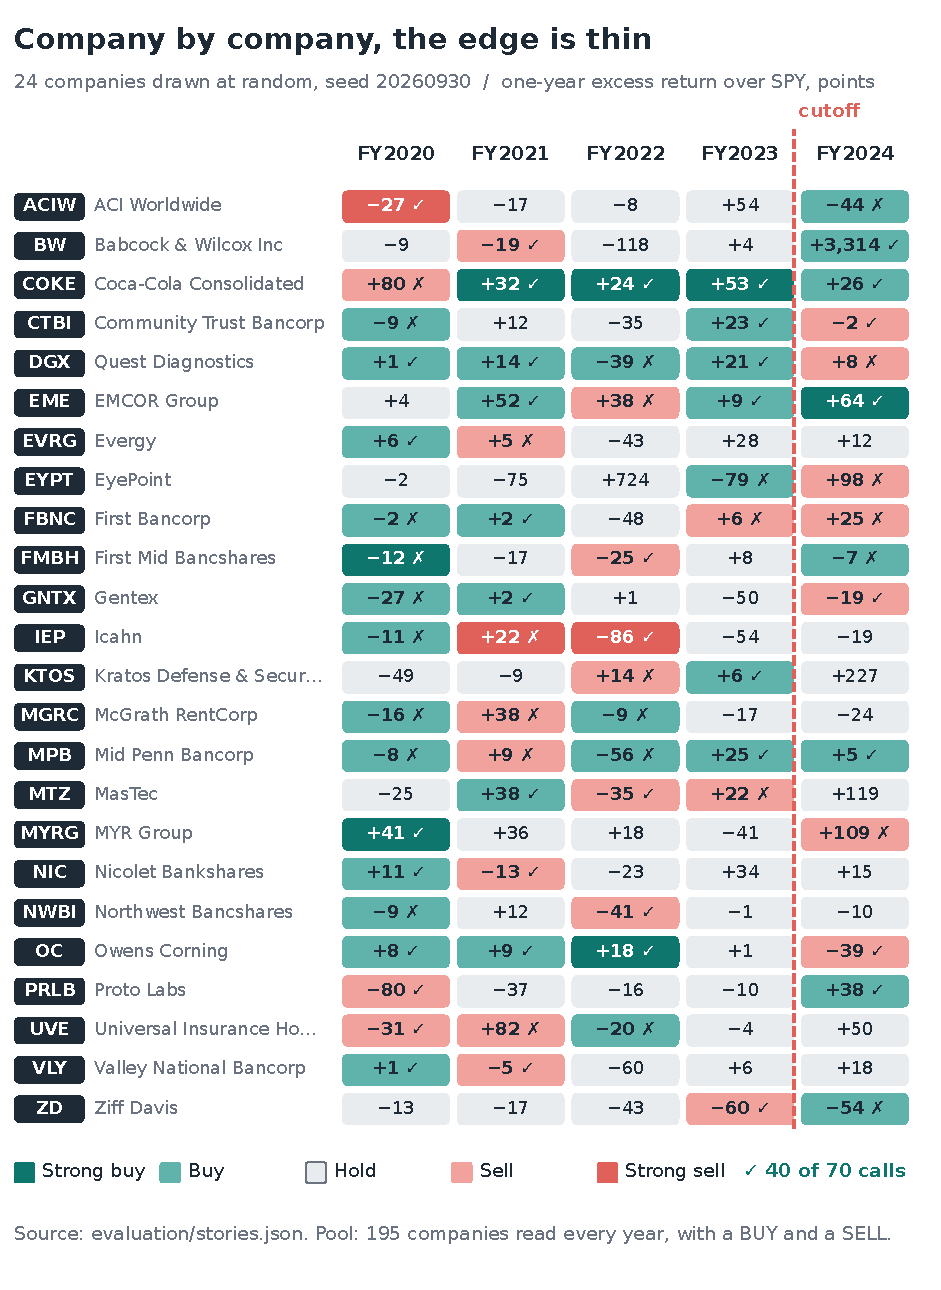
\includegraphics[width=1\linewidth,height=\textheight,keepaspectratio,alt={A grid of 24 randomly drawn companies by five fiscal years, each cell coloured by verdict and labelled with the one-year excess return, with ticks and crosses for right and wrong calls.}]{figures/13-company-grid.pdf}
\caption{Company by company, the edge is thin. Colour is the verdict; the number is the
one-year return over SPY in percentage points; a tick marks a BUY that beat SPY or a SELL that
trailed it. The rule selects on verdicts, never outcomes. Because the median stock trailed SPY
in these years, SELL ticks come cheaply. Source:
evaluation/stories.json.}\label{fig:13-company-grid}
\end{figure}

\subsection{8.4 A ledger written in 2025}\label{a-ledger-written-in-2025}

The strictest evidence is the oldest. The 2025 scripts wrote their scores to disk in May and
June 2025, after the model's cutoff and before any of the returns they might predict. They are
a ledger, and they need no argument about training data (Figure 14). Their dates come from file
timestamps, not a sealed archive, and I had looked at the first result before writing the test.

\textbf{Resemblance to great companies pointed the wrong way.} Across 1,766 companies, the
higher the 2025 compounder score, the worse the next year: Spearman \ensuremath{-}0.14, p = 0.0001. The top
fifth trailed SPY by 17.8 points on average; the bottom fifth beat it by 18.6. A sensible idea,
carefully applied, failed its first year. One plausible reason, untested, is that looking like
a past winner was already in the price. The original ambition was about decades, which one year
cannot settle.

\textbf{The contrarian score and the options calls showed nothing.} Spearman +0.01 (p = 0.71)
for the contrarian score; calls minus puts +2.8 percentile points (p = 0.54) over six months
for the options ideas.

\begin{figure}[!htbp]
\centering
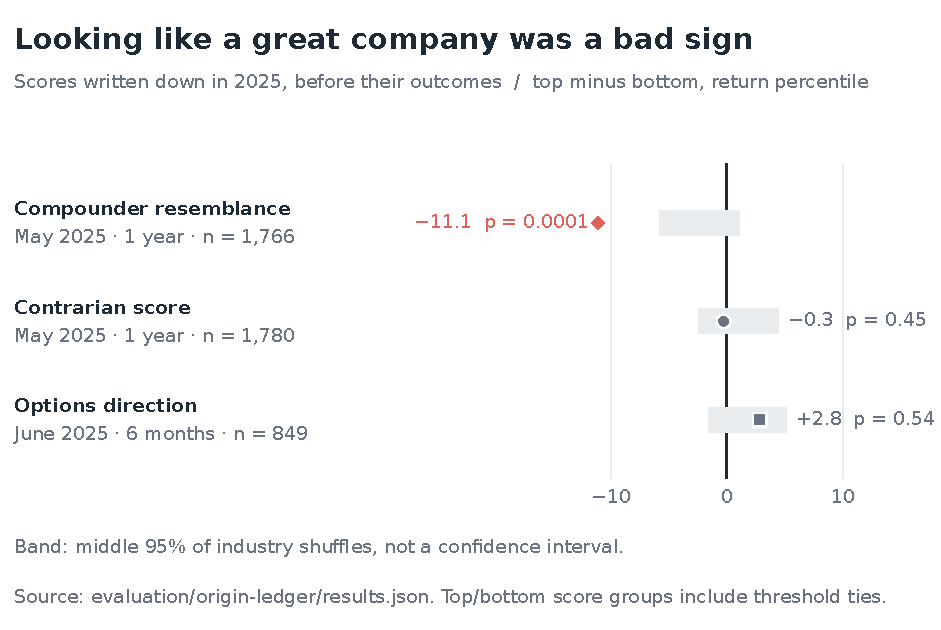
\includegraphics[width=1\linewidth,height=\textheight,keepaspectratio,alt={Three 2025 scores against their industry-shuffle bands: compounder resemblance far below its band; contrarian and options scores inside theirs.}]{figures/14-dated-ledger.pdf}
\caption{Looking like a great company was a bad sign. Top fifth minus bottom fifth of each 2025
score (calls minus puts for options), in percentile points of return, against the middle 95\%
of 10,000 industry-preserving shuffles. Source:
evaluation/origin-ledger/results.json.}\label{fig:14-dated-ledger}
\end{figure}

These are not EON's verdicts. Across 1,054 companies scored by both, the compounder score and
EON's verdict are almost unrelated (Spearman 0.05).

\subsection{8.5 A ledger written in February 2026}\label{a-ledger-written-in-february-2026}

EON left a ledger of its own. The Asymmetric Options V4 scan of 25--26 February 2026 recorded,
for 1,415 companies, a directional bias and an asymmetry score, six months before the outcomes
it would be graded on. I wrote the test before running it (Figure 15).

\begin{figure}[!htbp]
\centering
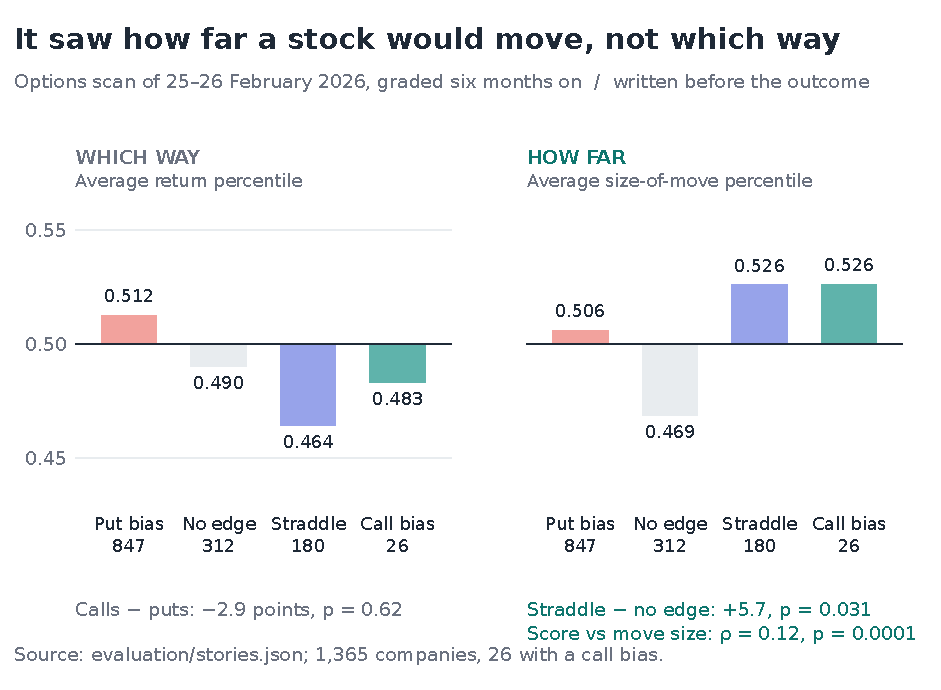
\includegraphics[width=1\linewidth,height=\textheight,keepaspectratio,alt={Two panels of bar charts by options bias: average return percentile, which barely differs, and average size-of-move percentile, which is higher for straddle and call-bias names.}]{figures/15-options-ledger.pdf}
\caption{It saw how far a stock would move, not which way. Six-month outcomes for 1,365
companies, by the bias the scan recorded in February 2026. Left: direction, as the average
percentile of excess return. Right: magnitude, as the average percentile of the absolute excess
return. Source: evaluation/stories.json.}\label{fig:15-options-ledger}
\end{figure}

On direction, the scan had no skill. Stocks marked for calls did no better than stocks marked
for puts (\ensuremath{-}2.9 percentile points, p = 0.62); put-bias stocks in fact beat SPY slightly more
often than the rest. On magnitude, it did. Its asymmetry score correlated with the size of the
move, up or down (Spearman 0.12, p = 0.0001), and stocks marked ``straddle'', the model's way
of saying something big will happen, moved more than those marked ``no edge'' (p = 0.031).

This is the cleanest positive result in the project, and it is the modest kind. A model reading
a 10-K can tell which companies are fragile, levered, dependent on a binary event, or opaque,
and those companies move more. It cannot tell which way. That is what an options trader would
call volatility, and it is already in the price of options.

\subsection{8.6 What the tests say together}\label{what-the-tests-say-together}

Graded with hindsight, the model looked like an analyst. Graded on what it could not have
known, it looked like a careful reader with a small, fading edge, one bad idea and one modest
talent. The evidence has limits that apply throughout: every clean result comes from roughly
the same eighteen months; the universe was drawn from companies still listed in 2026; industry
is controlled but size, value, quality and momentum are not; extraction and the model's facts
are unaudited; and returns are not trades. Section 11 is what the paper does about that.

\FloatBarrier
\clearpage
\section{Part III · What it taught}\label{part-iii-what-it-taught}

\section{9. How the model went wrong}\label{how-the-model-went-wrong}

The most useful findings in this project are not about stocks. They are about how a fluent
language model fails when it is asked to do a job thousands of times (Figure 16).

\begin{figure}[!htbp]
\centering
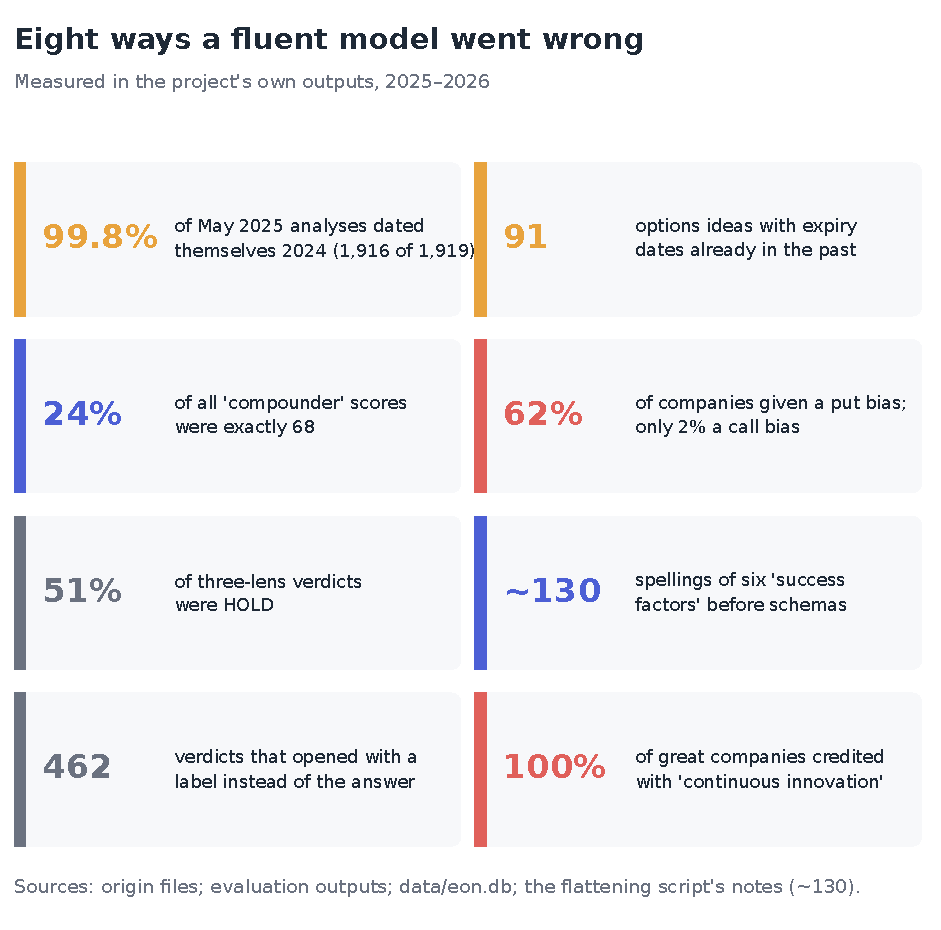
\includegraphics[width=1\linewidth,height=\textheight,keepaspectratio,alt={Eight cards, each with a large number: 99.8\% of analyses misdated, 91 expired option dates, 24\% of scores exactly 68, 62\% put bias, 51\% HOLD, about 130 spellings, 462 mislabelled verdicts, and 100\% innovation.}]{figures/16-shortcomings.pdf}
\caption{Eight ways a fluent model went wrong. Each number is measured in the project's own
stored outputs. Sources: the origin files; evaluation outputs; data/eon.db; the flattening
script's notes.}\label{fig:16-shortcomings}
\end{figure}

\textbf{It did not know what day it was.} Run in May 2025, the model dated 1,916 of 1,919
analyses 2024, a year behind, and proposed 91 option expiries that had already passed. It
reasons from its training-time present unless told otherwise. EON's later workflows stamp dates
in code.

\textbf{It may remember the future.} A model trained after the events it is asked to judge can
borrow from them without saying so. A search of every reading for terms with known first-use
dates found no careless leaks: the Inflation Reduction Act appears in 300 readings, never in
one of a filing written before the law. But a verdict nudged by memory leaves no trace in its
prose.

\textbf{Its numbers are less precise than they look.} A quarter of all compounder scores were
exactly 68. A 0--100 scale that behaves like a four-point one invites false precision. The
later workflows use anchored scales, each defined at 0, 5 and 10.

\textbf{It leans.} It holds half the time. Asked to look for tail risk, it found it in 62\% of
companies and upside in 2\%. The framing of a question shapes the answer's direction as much as
the evidence does.

\textbf{It favours platitudes and the famous.} It credited ``continuous innovation'' to every
great company, and its contrarian scan's hidden gems included Apple, Microsoft and Nvidia.

\textbf{It drifts in format.} Without a schema, six factors took 130 spellings. With one, 462
verdicts still opened with a label (``Overall investment recommendation: \ldots{}'') instead of
the answer, and conviction arrived in half a dozen phrasings. Every parser must expect this.

\textbf{It cannot always add.} CSPP stopped trusting its arithmetic and recomputed every total
in code.

\textbf{It sometimes stops.} One large filing hung a call for about two hours without an error.
Every call now has a watchdog.

\textbf{It values without prices.} Apple's SELL rests on a ``highly stretched valuation'', but
a 10-K contains no current share price. The model supplies one from memory, which is exactly
the channel through which hindsight can leak.

\section{10. Why it was worth doing}\label{why-it-was-worth-doing}

EON was never going to rival Citadel, Point72 or the Medallion Fund. Those firms buy data
nobody else has, trade in milliseconds, employ hundreds of researchers, and move capital at
scale. Medallion is famous for short-horizon statistical patterns, not opinions about annual
reports. A 10-K is the most public document a company produces. Thousands of professionals read
the important ones on the day they are filed; whatever it says is in the price within hours. A
machine reading the same text a year later, on free quotas, was not going to find money lying
on the pavement.

It was worth doing anyway, because it was three projects at once.

\textbf{As a finance project,} it turned a vague question (can reading annual reports well tell
you anything?) into a measurable one, and taught the details that make such measurements
honest: excess returns and their benchmark, industry composition, survivorship, the difference
between an average and a rank, one stock deciding a mean, and above all look-ahead. The answer
was humbling in the right way: what a filing says is largely known, and what it signals most
reliably is risk, not direction.

\textbf{As an AI project,} it measured a language model at scale, on the same task, thousands
of times, and caught it misdating its work, drifting in format, clustering its scores, leaning
bearish when asked about risk, and possibly remembering the future. Those are not failures of a
particular prompt. They are properties of fluent models, and they only show up in volume.

\textbf{As a systems project,} it forced real engineering under a hard constraint:
cross-process locks, key rotation, leases and heartbeats, crash recovery, a database built to
survive two weeks of interruption, two operating systems, two interfaces, and an alarm that
works while you sleep. None of that was planned. Every piece answers a failure that happened.

And it left something no one else has: 29,375 answers written down with their dates, a method
for testing them honestly, and a bet.

\section{11. The bet}\label{the-bet}

Every lesson in this paper points to one practice: write the verdict down, with its date,
before the future arrives. So the paper makes a forecast of its own (Figure 17).

\begin{figure}[!htbp]
\centering
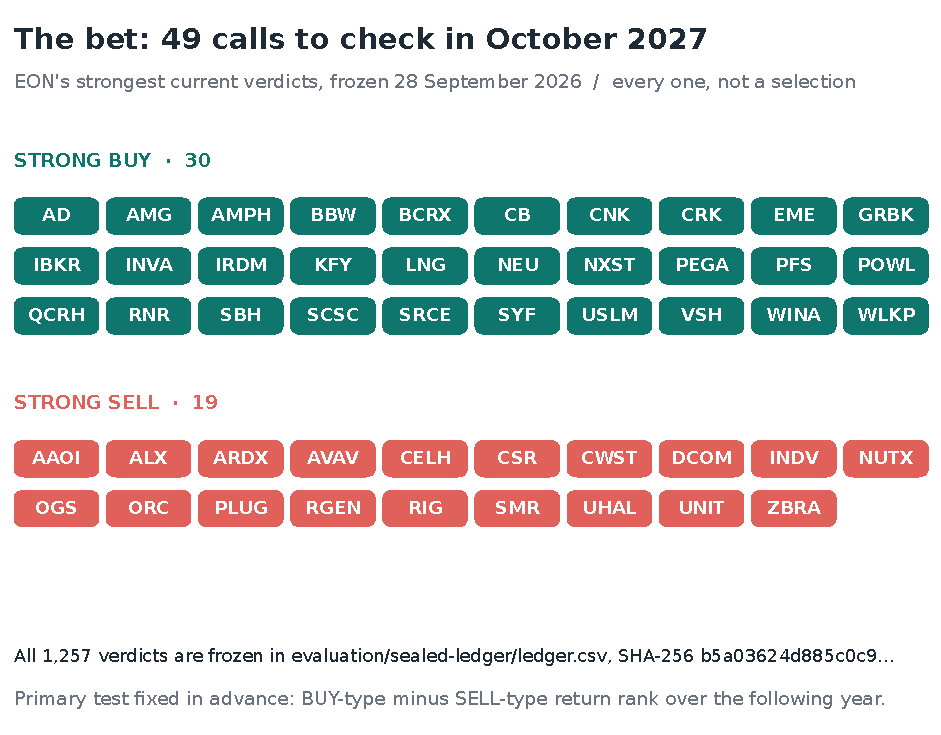
\includegraphics[width=1\linewidth,height=\textheight,keepaspectratio,alt={Ticker tiles for all 30 STRONG BUY and 19 STRONG SELL verdicts frozen on 28 September 2026.}]{figures/17-sealed-bet.pdf}
\caption{The bet: 49 calls to check in October 2027. EON's latest verdict on each of 1,257
companies, frozen on 28 September 2026 with their prices, and graded one year after
publication. The tiles are every STRONG BUY and STRONG SELL, not a selection. Source:
evaluation/sealed-ledger/.}\label{fig:17-sealed-bet}
\end{figure}

The ledger holds EON's most recent verdict for each of 1,257 companies: 634 HOLD, 341 BUY, 233
SELL, 30 STRONG BUY and 19 STRONG SELL. The whole file is fixed by its SHA-256 fingerprint,
which begins b5a03624d885c0c9. The test was chosen in advance: BUY-type minus SELL-type
percentile rank of one-year return over SPY, from the first close after 30 September 2026. Many
of these verdicts are already a year old, since they read filings from early 2025; that is part
of the test.

The next vintage should do better than a frozen file on one laptop. Read the fiscal 2025
reports now, with the same model and prompt; store each reading with the filing's identifier, a
hash of the text the model saw, the prompt version and the time; pin the model, because a new
model has a new cutoff and turns clean evidence back into hindsight; tell it the date; and
publish the fingerprint somewhere public before the returns arrive.

\section{12. Conclusion}\label{conclusion}

I set out to build a patient reader. It took five versions and seventeen months, and most of
the work was not reading at all. It was waiting for midnight, printing web pages, keeping two
dozen workers from colliding, and making sure nothing was lost when something broke.

The reader works. It is specific, tireless and consistent enough to be counted. Counting it
produced a result that looked like foresight, and arranging the evidence by what the model
could have known took most of that away. What remains is modest and real: a small edge in its
BUY calls, a sense of which companies will move a lot, and a clear view of how a fluent model
goes wrong.

The newspaper the model read ends in January 2025. Everything after that has to be read the
ordinary way, one day at a time.

\textbf{Write the question once. Keep the answer with its date. Let the next year answer back.}

\FloatBarrier
\clearpage
\section{Appendix A: methods}\label{appendix-a-methods}

\textbf{Scope.} One reading per ticker and fiscal year, the first stored. Of 6,653 such
readings, 6,651 were made with Gemini 2.5 Flash; two made with Gemini 3.5 Flash are excluded. A
usable observation needs a parsed verdict, a filing date and prices: 6,203 readings of 1,309
companies.

\textbf{Returns.} Entry at the first close strictly after the filing date. Excess return is the
change in adjusted close over 126, 252 or 504 trading sessions minus SPY's change over the same
dates, in percentage points, not annualised. For the ledgers, entry follows the recorded
reading date. Prices are a frozen Yahoo Finance snapshot through 28 September 2026; the largest
outlier was checked against Nasdaq.

\textbf{Samples.} ``Before the cutoff'' means the return window closed before 31 January 2025.
``After the cutoff'' means the filing was published after it.

\textbf{Spreads and ranks.} The mean spread is the BUY-group average excess return minus the
SELL-group average. The rank spread uses each reading's percentile within its fiscal year, so
no single stock can dominate.

\textbf{Permutation tests.} Verdicts are shuffled 10,000 times within fiscal years, and
separately within fiscal-year-and-industry groups (industry from a February 2026 FactSet
snapshot; single-reading groups dropped). Two-sided p-values measure distance from the shuffled
mean, with a plus-one correction; 0.0001 is the floor.

\textbf{What was fixed in advance.} The historical one-year and post-cutoff six-month tests
were specified first. The post-cutoff one-year test, the rank statistic and the anachronism
search were added after earlier results were seen. The verdict ladder, company grid and
February 2026 options test follow \passthrough{\lstinline!stories-config.yaml!}, written before
they were run. None is adjusted for multiple comparisons.

\textbf{Ledgers.} The 2025 scores are read from the origin project without modification;
compounder dates come from file modification times, other dates from filenames. The February
2026 options scan uses each reading's stored timestamp.

\textbf{Pipeline measurements.} Page counts, characters and extraction times come from 40
randomly sampled cached 10-K PDFs; markup ratios and XBRL counts from 17 raw EDGAR 10-K files.
Tokens are estimated at four characters each.

\section{Appendix B: related work and references}\label{appendix-b-related-work-and-references}

Sarkar and Vafa show that pretrained language models carry information about periods after
their nominal analysis date, and test for it with events that should be unpredictable; the
anachronism search in Section 9 is a simple instance. Glasserman and Lin measure look-ahead
bias in model-scored news sentiment and reduce it by removing company names. Lopez-Lira and
Tang find that model readings of headlines predict next-day returns; EON reads a different
document over a longer horizon, and its results are not a replication.

\begin{itemize}
\tightlist
\item
  Glasserman, P. and Lin, C. (2023). \emph{Assessing Look-Ahead Bias in Stock Return
  Predictions Generated by GPT Sentiment Analysis.} arXiv:2309.17322.
\item
  Google. \emph{Gemini 2.5 Flash model documentation}, knowledge cutoff January

  2025. ai.google.dev/gemini-api/docs/models/gemini-2.5-flash.
\item
  Lopez-Lira, A. and Tang, Y. (2023). \emph{Can ChatGPT Forecast Stock Price Movements? Return
  Predictability and Large Language Models.} arXiv:2304.07619.
\item
  Sarkar, S. K. and Vafa, K. (2024). \emph{Lookahead Bias in Pretrained Language Models.} SSRN
  4754678.
\item
  US Securities and Exchange Commission. \emph{EDGAR fair access policy}: no more than ten
  requests per second.
\end{itemize}

\section{Appendix C: reproduction}\label{appendix-c-reproduction}

The Markdown is the editorial source; LaTeX and PDF are generated from it.
\passthrough{\lstinline!BRIEF.md!} sets the editorial standard,
\passthrough{\lstinline!figures.md!} documents every figure,
\passthrough{\lstinline!graphics.md!} briefs the commissioned illustrations, and
\passthrough{\lstinline!revision-notes.md!} records every change and open question.

{\def\LTcaptype{table} % do not increment counter
\par\addvspace{8pt}\noindent\begin{minipage}{\linewidth}\small
\begin{tabular}{@{}
  >{\raggedright\arraybackslash}p{(\linewidth - 2\tabcolsep) * \real{0.5500}}
  >{\raggedright\arraybackslash}p{(\linewidth - 2\tabcolsep) * \real{0.4500}}@{}}
\toprule\noalign{}
\begin{minipage}[b]{\linewidth}\raggedright\bfseries
Path
\end{minipage} & \begin{minipage}[b]{\linewidth}\raggedright\bfseries
Role
\end{minipage} \\
\midrule\noalign{}


\passthrough{\lstinline!eon/data/sources/sec/!} & Download, Chrome conversion, extraction, SEC
queue \\
\passthrough{\lstinline!eon/ai/!} & Prompts, key manager, request queue, Gemini provider \\
\passthrough{\lstinline!eon/ui/database/!} & Repository, migrations v001--v014 \\
\passthrough{\lstinline!eon/ui/services/batch\_queue.py!} & Leases, heartbeats, quota waits,
alerts \\
\passthrough{\lstinline!evaluation-config.yaml!} & Main evaluation and its amendments \\
\passthrough{\lstinline!origin-ledger-config.yaml!} & 2025 ledger test \\
\passthrough{\lstinline!stories-config.yaml!} & Ladder, company draw, February 2026 options
test \\
\passthrough{\lstinline!sealed-ledger-config.yaml!} & The bet \\
\bottomrule\noalign{}
\end{tabular}
\end{minipage}\par\addvspace{8pt}
}

\par\noindent\begin{minipage}{\linewidth}

From the EON root:

\par\noindent\begin{minipage}{\linewidth}
\begin{lstlisting}[language=sh]
python docs/whitepaper/evaluate_backtest.py
python docs/whitepaper/evaluate_origin_ledger.py
python docs/whitepaper/evaluate_stories.py
.venv/bin/python docs/whitepaper/measure_pipeline.py
python docs/whitepaper/prepare_figure_data.py
python docs/whitepaper/render_figures.py
python docs/whitepaper/validate_paper.py
python docs/whitepaper/build_paper.py --pandoc /path/to/pandoc
cd docs/whitepaper && tectonic -X compile eon-whitepaper.tex
\end{lstlisting}
\end{minipage}\par

\end{minipage}\par

The evaluators open databases read-only and use saved prices; the origin evaluator reads
\passthrough{\lstinline!stock\_stuff\_06042025/10K\_automator!} without changing it. The sealed
ledger's script refuses to run twice.

\emph{Prepared from the EON repository and its predecessors, their databases and files, and a
frozen price snapshot. Negative and inconclusive results are retained. Research, not investment
advice.}

\end{document}
